% !TeX root = ../thuthesis-example.tex

\chapter{引言}

\section{研究背景与意义}
互联网、物联网、云计算等计算机科学技术经过长时间的共同发展与不断融合,
积累了规模庞大、种类繁多的海量数据,涉及计算机科学、宏观经济、
军事科技、医疗卫生等诸多领域。根据统计,谷歌每天处理分析超过数百
PB的数据,脸书每个月产生超过10PB的日志数据,百度每天处理将近100PB
的数据,而淘宝每天可以产生数十个TB的数据。截至2012年,
技术上可在合理时间内分析处理的数据集大小单位为艾字节(EB)。
在这些海量数据之中,有一类按照数据生成的时间顺序,把同一个变量或
记录的数据值,或者高维数据的一个元组,排列而成的记录数据信息,
被称为时间序列。时间序列是工业界应用广泛的、与时间维度相关的
高维数据,也是数据挖掘技术的一种主要研究对象。

大部分时间序列数据中数据点会随着时间的变化而产生一定的变化规律,
其中某些规律在同一个时间序列中多次重复出现,这类规律称为模式。
时间序列中蕴含着多种多样的模式,挖掘出时间序列中蕴含的模式,
既可以为未来的决策提供理论与数据支持,又可以检测、判断、预防突发
错误的出现,指导实际生产。因此,时间序列模式挖掘是时间序列分析和
数据挖掘中的重要组成部分。在多样化的模式中,对称模式因为具有独特的
物理意义,在多种应用场景的时间序列数据中大量出现,具有重要的
研究价值。然而,由于时间序列数据的特殊性,对称模式的挖掘也
存在许多困难。

从数学角度,判断序列具有对称性的方式十分简单,确定对称中心,
并计算中心一侧序列是否为另一侧的镜像即可。图~\ref{fig:symmetric_string}
展示了对称字符串序列示意图,该序列在“D”两侧的子串互为镜像,
则为对称(回文)字符串序列。然而,时间序列的对称性并不像回文字符串序列
的对称性具有非常严格的数学定义,并不存在严格统一的对称中心。
图~\ref{fig:no_symmetic_center}展示了血压测量中力感测电阻器(FSR)
信号的变化示意图,尽管在物理意义上一次心跳过程的压缩和舒张阶段时间序列
具有对称性。然而,由于压缩阶段和舒张阶段的时长不一致,
采集点的个数不同,其对称中心并不严格位于时间的中点。
因此,在计算序列对称性时,不能简单地查找对称中心并根据对称中心将时间序列
分段,以免计算的对称度不准确。除此之外,由于物理设备、数据采集和数据传输
中遇到的问题,实际应用场景中的时间序列可能不是等间隔采样的,导致不同阶段
的数据点密度不一致,这种情况同样会造成对称中心点的不确定性。
\begin{figure}[t]
  \centering
  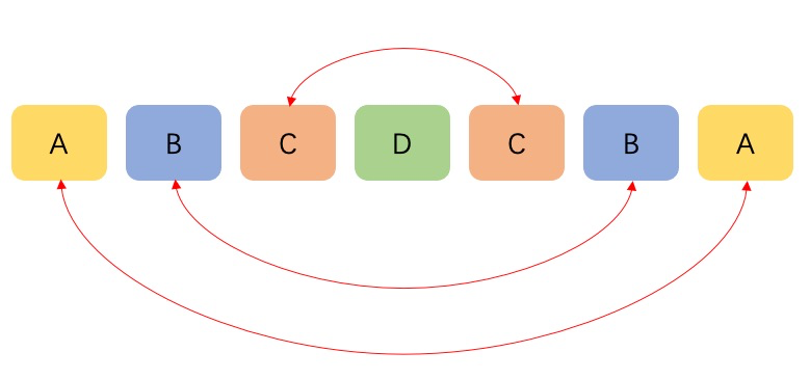
\includegraphics[width=0.86\linewidth]{symmetric_string.png}
  \caption{对称字符串序列}
  \label{fig:symmetric_string}
\end{figure}

\begin{figure}[h]
  \centering
  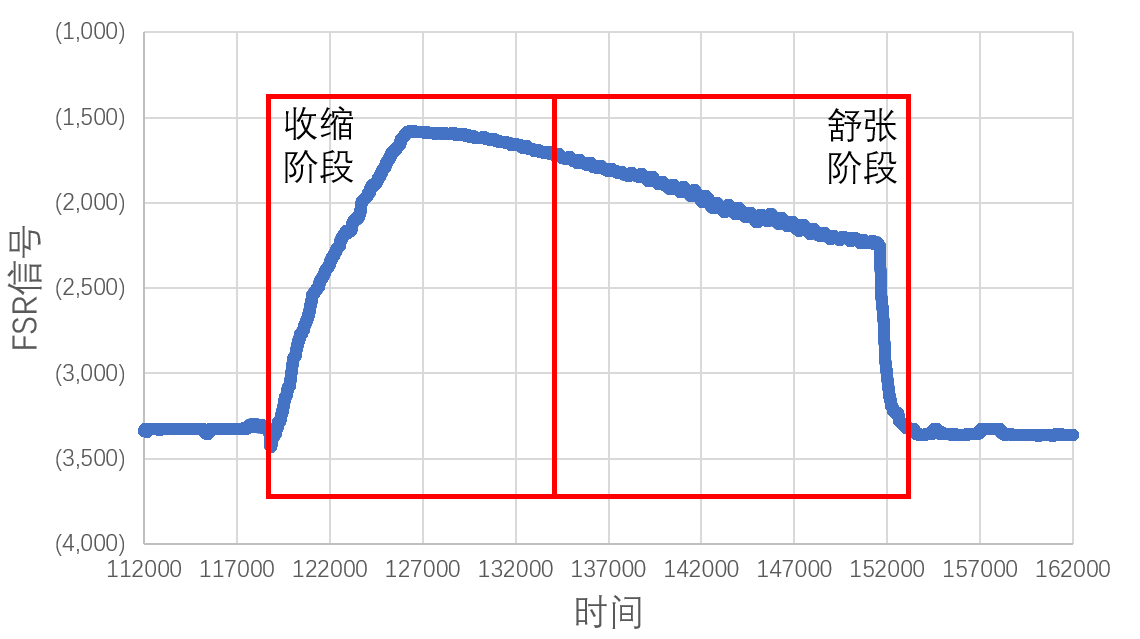
\includegraphics[width=0.86\linewidth]{no_symmetic_center.png}
  \caption{对称时间序列反映无严格对称中心的案例}
  \label{fig:no_symmetic_center}
\end{figure}

此外,由于采样频率不同以及数据随机性较大,时间序列在对称性匹配过程中
不可避免的存在一些失配现象。图~\ref{fig:mismatch}展示了某辆挖掘机
在作业过程中动臂提升工况的变化示意图,该序列为一次挖掘作业的动臂提升工况
时间序列,具有物理上的对称性。然而,由于抬臂阶段产生了红框所示的数据采集
缺失,导致动臂提升工况时间序列的抬臂和降臂阶段并不完全匹配。因此,
在对称模式的挖掘过程中,需要考虑到因为部分失配导致的对称度计算结果偏差问题。

除了利用对称中点截断时间序列计算对称性之外,使用原始时间序列和
其反转时间序列的相似性来度量对称性也是一种常见的方法。然而,
时间序列的对称性与时间间隔、序列模式和数据特征密切相关。在实际工业场景中,
原始和反转时间序列在时间线上不对齐的情况时有发生,不存在严格的一一对应关系,
使用传统的匹配方法,无法进行全局匹配度量。图1.4对比了某辆运煤车在行驶过程
中生成的纬度时间序列不同的匹配方式,可以看出,一一对应的匹配方式存在大量
的未对齐点,由此计算得到的对称度明显偏大。而全局匹配方式则应该从全局匹配
角度为原始和反转时间序列上的每对点求得最佳匹配,从而使计算得到的对称度最高。
因此,需要立足于时间序列的时间和全局数据特征挖掘其子序列的对称性。
\begin{figure}
  \centering
  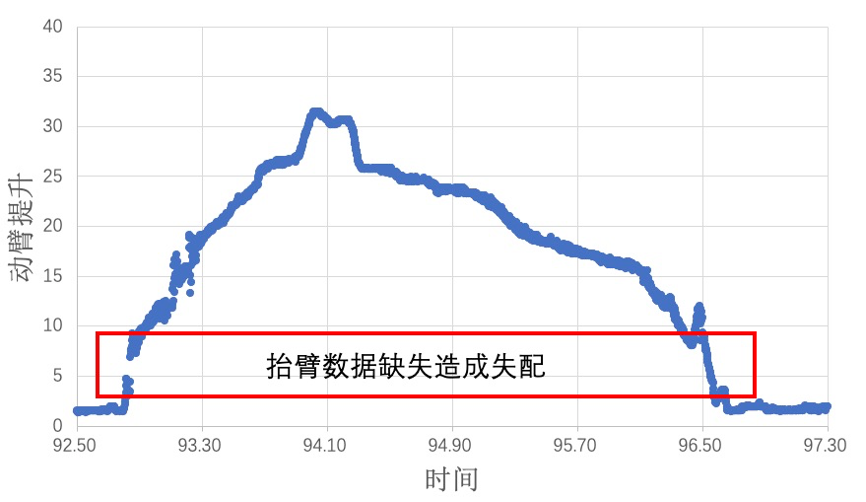
\includegraphics[width=0.86\linewidth]{mismatch.png}
  \caption{对称时间序列反映随机失配现象的案例}
  \label{fig:mismatch}
\end{figure}
\begin{figure}
  \centering
  \subcaptionbox{一一对应\label{fig:time_series_align-a}}
    {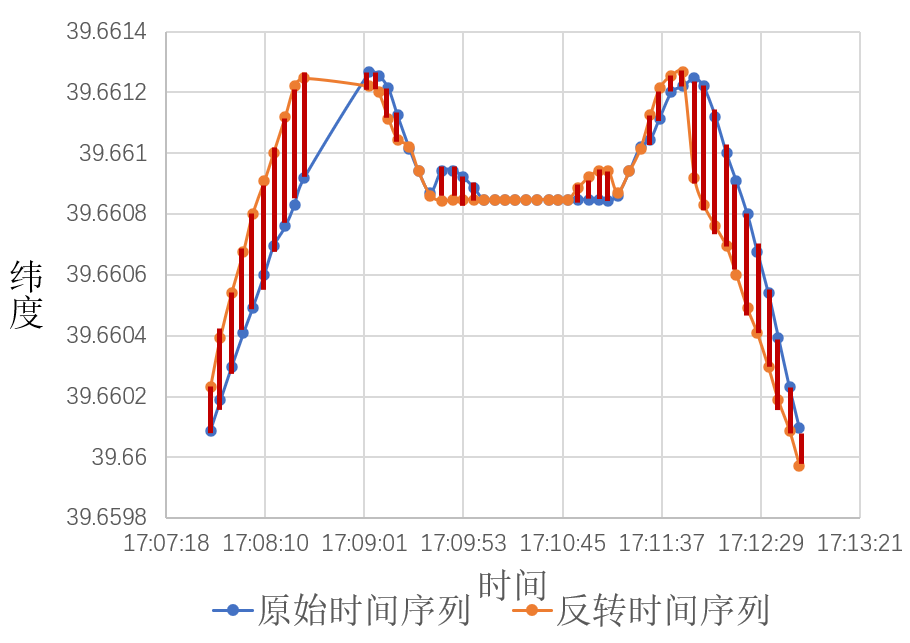
\includegraphics[width=0.43\linewidth]{time_series_align-a.png}}
  \subcaptionbox{全局匹配\label{fig:time_series_align-b}}
    {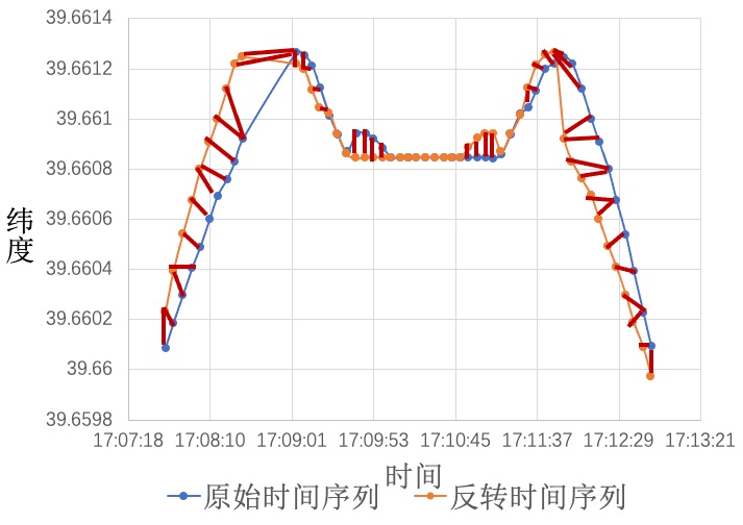
\includegraphics[width=0.43\linewidth]{time_series_align-b.png}}
  \caption{对称时间序列反映不对齐现象的案例}
  \label{fig:time_series_align}
\end{figure}

并且,给定时间序列的长度约束,挖掘出的对称子序列可能存在重叠情况,
从而导致后续数据分析和统计存在误差。图~\ref{fig:overlap}展示了挖掘机连续作业过程中
斗杆外摆工况变化的时间序列,该时间序列中的对称模式表示一次装车完成,
具有实际的物理意义。然而,尽管a、b、c都是具有对称性的对称子序列,
若把三者都识别为对称模式,不仅会因为重叠导致对称模式物理意义的不明确,
而且会使得最后统计的装车数量与真实数量有偏差。因此,需要根据时间序列中
对称子序列的分布,挖掘出不重叠的对称子序列集合。
\begin{figure}
  \centering
  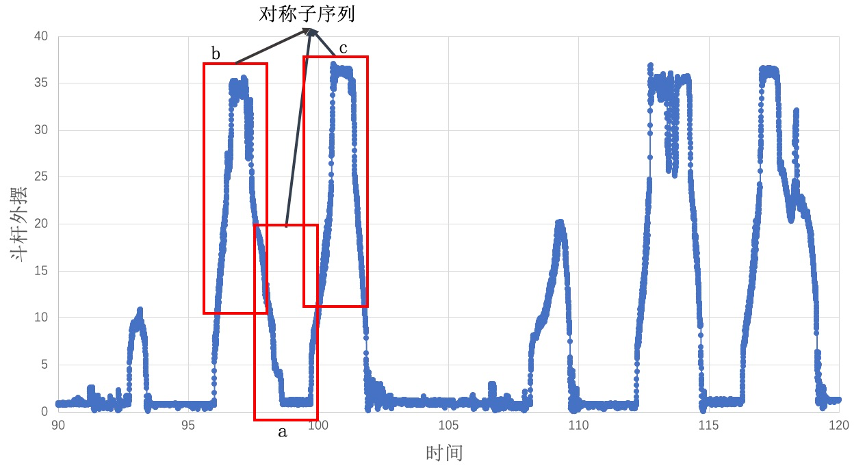
\includegraphics[width=0.86\linewidth]{symmetric_overlap.png}
  \caption{对称时间序列反映重叠现象的案例}
  \label{fig:overlap}
\end{figure}

总之,时间序列中的对称模式往往具有某种具体的物理意义,在血压监测图,
温度变化图和行车路线图等多种应用场景的时间序列数据中大量出现,挖掘
对称模式对于轨迹跟踪,作业分析,异常检测和序列预测都具有重要价值。
然而,时间序列的复杂性和不确定性为对称模式挖掘带来了诸多挑战。基于此,
本文提出了一种准确高效的时间序列对称模式挖掘方法,并将该方法扩展到了
流式数据场景,通过实验验证了本方法的应用价值。


\section{研究内容与贡献}
为解决上述问题,本文将研究一种完整高效的时间序列对称模式挖掘,具体包含
以下三个方面:
\begin{enumerate}
  \item 时间序列的对称性并没有标准的度量方法,现有的基于对称中心与
  原始和反转时间序列的方法都存在问题。不同于回文字符串,时间序列并
  不存在严格统一的对称中心,通过对称中心截取子序列度量对称性的方法
  其效果极不稳定。直接通过原始时间序列和其反转时间序列的相似性度量
  对称性的方法可以避免确定对称中心的问题,但是重复计算,时间不对齐等
  问题也会导致对称性度量结果偏大,从而影响对称模式挖掘结果的准确性。
  因此,如何定义一种准确高效的时间序列对称性度量方法成了首要的目标。
  \item 在全局时间序列上挖掘对称模式是一个多步骤的算法框架,
  不仅需要度量子序列的对称性,而且,对称时间序列并不要求原始时间序列
  和其反转时间序列完全相同,只需要两者的距离在指定阈值范围内即可。
  因此,本文需要通过计算阈值来挖掘出真正的对称子序列。此外,时间序列中
  蕴含的对称模式可能存在重叠,需要设计算法过滤重叠的对称子序列,
  从而挖掘出不重叠的对称子序列集合,即对称模式。
  \item 对于流式数据上的对称模式挖掘,由于无法提前预知时间序列的全貌,
  静态的时间序列对称性度量算法失效。本文将研究如何使方法满足流式或
  分布式计算场景要求。流式计算场景要求方法只对数据进行一轮遍历且
  可增量执行。此外,时间序列中很可能存在长度不同的对称模式,
  为保证挖掘的完整性,需要研究可以自适应调整时间窗口大小的算法。
\end{enumerate}

基于以上的研究内容,本文主要贡献如下:
\begin{enumerate}
\item 定义了对称子序列和对称模式。本文所挖掘的模式是关于中心点前后对称
的子序列模式,其对称性由原子序列和反转子序列的相似性进行度量。对称模式
在实际工业生产中非常常见,具有很高的应用价值。
\item 提出了静态时间序列对称模式的挖掘方法,并给出了具体的算法。
设定对称子序列的长度约束,采用区间动态规划算法计算出时间子序列的对称度,
然后使用由分布特征确定的对称度阈值分类得到对称子序列,最后根据获取数量
最多对称子序列的贪心策略,计算得到所有不重叠的对称模式。
\item 将对称子序列的挖掘算法扩展到了数据流上,每生成一个新的数据点,
实时计算出包含当前数据点的子序列对称性,根据对称性阈值及时筛选出对称子序列。
\item 研究了时间子序列对称性和窗口大小的关系,
分析建模了对称序列数据点差分的数据范围,并根据范围自适应调整窗口大小。
\item 本文采用了来自UCR和真实工业场景中的时间序列数据集在
挖掘对称模式的精确率、完整性以及时间开销方面进行了实验,
并与多种现有相关方法进行了对比。
结果表明:本文所提出的时间序列对称模式挖掘算法在挖掘效果方面表现最优,
同时在时间开销方面有着几乎最佳的性能。此外,本文对对称模式挖掘算法
进行了系统实现,把它们集成到IoTDB数据质量分析工具IoTDB-Quality中。
一方面,完善了IoTDB-Quality工具的功能,弥补了工具在时间序列模式挖掘
上的功能缺失。另一方面,通过挖掘出时间序列中的对称模式,工具可以继续
对时间序列进行分析预测和异常检测,进一步推动了IoTDB-Quality工具的应用。
\end{enumerate}

\section{论文组织结构}

本文共划分为 7 个章节,各个章节的组织内容如下所述:

第 1 章为引言部分,主要介绍了时间序列数据的特点和对称模式挖掘的挑 战,并据此引出本文的研究内容,最后总结了本文的工作内容和贡献。

第 2 章介绍并定义了本文涉及到的概念知识,即时间序列和对称模式。之后对国内外在序列相似性度量和模式挖掘上的研究进行了分类和阐述。

第 3 章提出基于对称子序列长度约束的对称模式挖掘方法,包括效率更高的对称度度量方法和根据数据分布特征自动确定对称度阈值的方法,最后根据贪心策略挖掘出数量最多且不重叠对称子序列组成的对称模式。

第 4 章对时间序列对称模式的挖掘进行了扩展。本文首先介绍了流式时间序列对称模式挖掘的难点,并对此扩展了动态规划的状态方程,提高了流式对称模式挖掘的效率。此外,本文还根据对称模式长度不一的问题,提出了可伸缩的自适应窗口挖掘更加完整的对称时间序列。

第 5 章通过一个人工数据集和三个真实工业时间序列数据集,在模式挖掘效果和时间性能等方面与现有方法进行对比分析,并通过多个数据集,在模式挖掘完整性上与现有方法进行比较验证。

第 6 章介绍了对称模式挖掘方法的系统实现。首先介绍了方法集成的目标工具 IoTDB-Quality,之后详细介绍了方法在工具上的具体实现和应用,以及给工具带来的意义。

第 7 章对本文的工作进行分析总结,并指出了未来工作的主要方向。 
